\chapter{Web assignment mirroring}
\label{sec:mirroring}

In this chapter, we are describing implementation and workflow of assignments mirroring in Courses 2 Learning Management System. This system offers students to submit their solutions of assignment via URLs which may be helpful on some courses, such as Modern Approaches to Webdesign course. During this course, student has to create multiple web pages which can be written in any web programming language. Since any student can choose any tool he wants, these web pages are usually stored on his own server. Here we present an algorithm of backing up these files on our servers.

\section{Motivation}
As it was said, students in some courses taught in the Courses 2 Learning Management System allow the students to submit their solutions as an URL address of their web site. This approach brings many advantages, for example students are allowed to choose the programming language and framework that suits them the best. For example, Modern Approaches to Webdesign course is not directly requesting the students to use specific languages rather than choose their own and let them focus on semantics rather than on learning a new tools.

The main disadvantage of this approach is that these submitted projects can not be hosted on servers at our Faculty for multiple reasons. We currently do not offer hostings other than for PHP programming language but many students choose different versions of this languages or go with other choices such as Python or Ruby on Rails. These require full virtual server for every students and may be hard to maintain for the teachers. Therefore we allowed students to host these web design projects on their own servers.

This approach is very beneficial for students and is a result of a long evolution. We want to continue using this approach but we needed some tools to improve it. For example, after these web design projects are submitted, students still can develop and edit their projects before or after evaluation by the teacher which is not a good thing. We also want to back up these projects for future use, for example to show them as examples for next year students.

So, we decided to implement mirroring of these assignments submitted by URLs. Our goal is to preserve most of the functionality and store them on our server as plain HTML, CSS or JavaScript documents. We do not want to execute script written in server side programming language, we only want to store the generated files.

This is however a very hard problem to implement well. Therefore it is needed to mention, that we do not expect these functionality to work on complicated sites written in modern JavaScript frameworks such as Angular or Node.js since most of the students wont use them or we can restrict usage of modules which could prevent us to backing up these sites correctly.

There is also one more thing we needed to do. Web pages often include logging in with username and password. First version of our algorithm could not back up pages shown after logging in which we saw as a major problem. We therefore decided to implement an algorithm, which could do it. Our presented algorithm can log in with username and password provided by the student and back up sites shown after log in also.

In the next sections, we describe process of mirroring these assignments, explain many problems we had to overcome, important details and provide some examples.

\section{Initialization}
First part of assignments mirroring process is submitting an assignment by the student. This is done as usual, in assignments module of the Courses 2 Learning Management System. The students submits his URL of an assignment which is then stored in database as a submission in \texttt{assignment\_submission} table as seen on Appendix A. This is the only action done directly by Courses 2 system. For reasons explained in \ref{sec:technology} we decided to build rest of this algorithm as a separate module which can be published on different server or virtual server.

\section{Mirroring}
After the submission is uploaded, it is ready to be mirrored. In this section we at first describe technology we used, modulation we choose and then explain thru the flow of this algorithm. Mirroring part of this algorithm is build as a separate module located in \texttt{webclone/cron} directory.

\subsection{Technology, pros and limitations}
\label{sec:technology}
For building a mirroring module, we decided to use PHP programming language. First versions of our mirroring were developped in Python, which provided excellent performance and fast development but it brought many more dependencies to system as a whole so we decided to use technologies we were already using. 

Usage of PHP for tasks such as this brings some disadvantages that must be overcomed. Most importantly, PHP is not build for supporting of asynchronous tasks. Usual flow of PHP application is that browser sends a request, web server starts PHP application and sends its result back to the browser. This flow, however can not be used for web site mirroring. Mirroring is a kind of task, which has to be executed asynchronously, independently of a browser or any request. It also has to be finished regardless of length of a task.

There is one commonly used solution for this problem, \texttt{cron} unix command. \texttt{Cron} is the system process which will automatically perform tasks for you according to a set schedule. The schedule is called the crontab, which is also the name of the program used to edit that schedule \cite{crontab}. We can set a \texttt{cron} command, to execute a given PHP endpoint every minute and set maximum running time of a script for one minute. This way we can constantly execute background jobs needed for mirroring.

Second important problem is, that with usage of cron, at least one of PHP workers is occupied. Web server we use, Apache 2, creates limited number of PHP workers for a website. We do not want to create any problems, such as lack of workers for requests for Courses 2, so we decided to create a separate module which takes care of mirroring. This module can be built as a separate virtual host (see \cite{apachepocket}) on a server with its own workers and processing. This way, we prevent any deadlocks in system.

We also build separate module for serving of these mirrrored websites, which will be described in \ref{sec:serving}. This module is also separated for security reasons and must have its own domain. Since JavaScript can access any cookies located under the same domain, and this JavaScript is created by the students, on their original website and mirrored on orurs, we could not run this module under \texttt{courses.matfyz.sk} domain. It could lead to a potential huge security flaw.

\subsection{Data model and filesystem}
\label{sec:filesystem}
To understand how this algorithm works, we at first need to understand its filesystem and data model used for saving mirrored files. 

\paragraph{Development of a fine tuned filesystem} for storing this web site documents, brought many problems. For best understaning, we continue with an example. Imagine that we are mirroring a web site \texttt{http://www.example.com/shop} and the current document, we are processing is located on \texttt{http://www.example.com/shop/product/bulb?q=yellow}. We want to mirror whole site structure under our url \texttt{http://our.site.dev/shop} and store these documents under \texttt{/home/www/htdocs/oursite/} folder. What is the proper way to store these documents?

\paragraph{Our first iteration} of this algorithm was using folders for storing files. We saved this document under \texttt{/home/www/htdocs/oursite/product/bulb?q=yellow} path and then set up Apache 2 Virtual Host to serve all documents located in \texttt{/home/www/htdocs/oursite/} under path \texttt{http://our.site.dev/shop}. This was a very straightforward approach.

Hovewer it brought many problems which could not be solved. For example, if the mirrored URL ended with a trailing slash, we had to delete this slash because Unix filesystems does not support filenames with trailing slashes. Then, we could set up Apache 2 virtual host to serve this file on both URL with and without trailings slashes.

But much worse situation was that two distinct documents were located in \texttt{http://example.com/abc} and \texttt{http://example.com/abc/}. This was a situation we could not solve with this straightforward solution.

\paragraph{Our second iteration} came with a concept of saving URLs into database and storing documents under hashed names. We decided to create a database model as seen of Figure \ref{webclonemodel}, which is to be explained later. For solving problem specified in example, we saved this file under random hash in the directory. Then, we extracted URL diff between the URL of the root site we want to mirror and URL of the current document. In example, it is \texttt{product/bulb?q=yellow} and store this as an URL of the document in \texttt{webclone\_document} table. This solution brought us a full range of advantages. For example, we could mirror redirect or error HTTP status codes and document URLs created with Apache 2 mod\_rewrite. On the other side, we had to create a file serving script, which is to be explained in Section \ref{sec:serving}.

\begin{figure}[h]
    \centering
    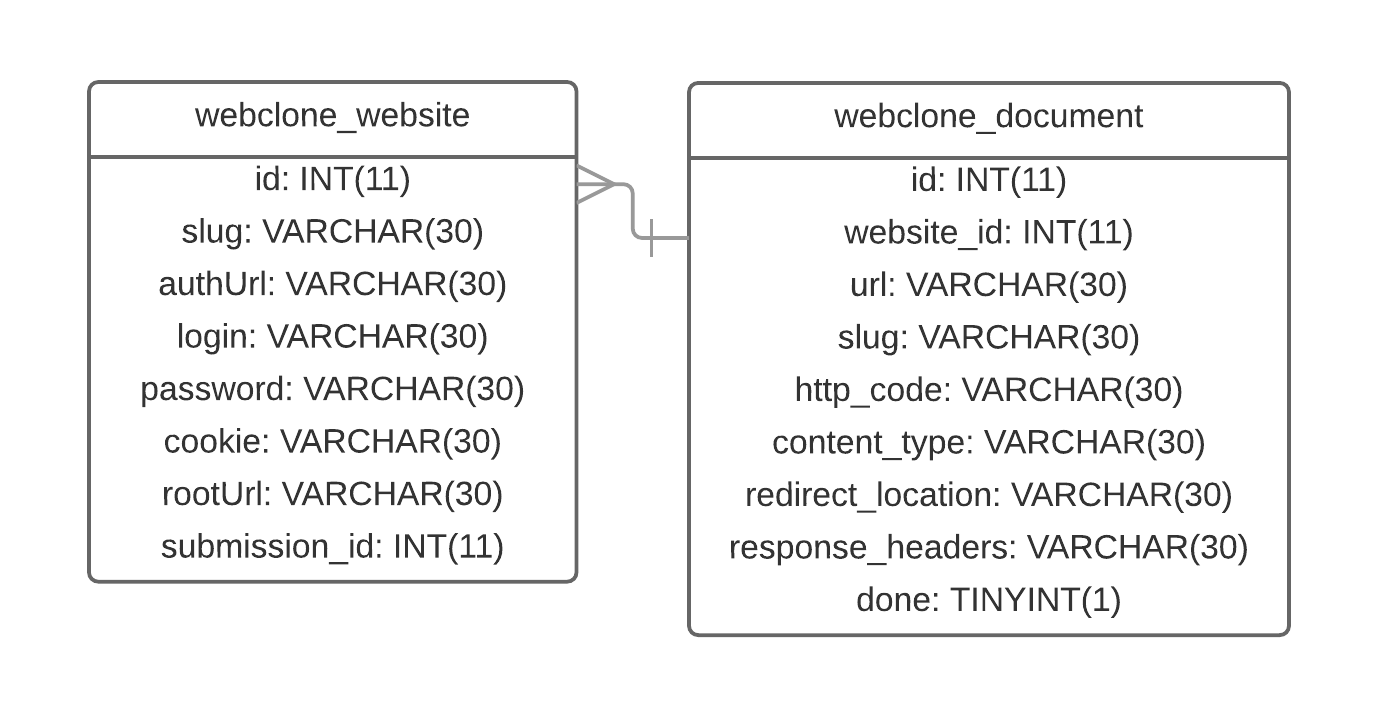
\includegraphics[width=\textwidth]{images/databaseWebclone.png}
    \caption{Database model of a webclone module.}
    \label{webclonemodel}
\end{figure}

As seen on Figure \ref{webclonemodel}, data model is split into two parts. The table \texttt{webclone\_site} represents a whole mirrored web site and the table \texttt{webclone\_document} represents a single document of this web site.

Fields in the table \texttt{webclone\_site}, slug is the name of the directory, under which the site structure is saved. AuthUrl, login, password and cookie fields are used for automated login explained in section \ref{sec:login}. RootUrl represents a root URL of the web site we are mirroring. In example above it would be \texttt{http://www.example.com/shop}.

In the table \texttt{webclone\_document}, we see reference to the \texttt{webclone\_site} as \texttt{website\_id}. Url is relative URL to the root site. In example above it would be \texttt{product/bulb?q=yellow}. Slug is used as a name of the real document file stored in directory. Http\_code is the Http code returned by original server when requesting this document. Content\_type is the content type returned by original server when requesting this document. Redirect\_location is specified, when returned Http\_code from the original server was redirect and this document was redirected under this location. Response\_headers are all of the Http Headers returned when requesting this document. And finally, done field means, that this document is already processed by our mirroring algorithm. This can be used as a queue of unprocessed document ordered by their IDs.

\subsection{HTTP Link replacement in mirrored documents}
\label{sec:linkReplace}
Now we need to look into replacing HTTP links in documents. In each document, whether it is HTML or CSS, we may find links to another documents in a form of \texttt{a}, \texttt{img}, \texttt{script} or other tags. As we want to mirror whole structure on the root server, we it is crucial to find a way to search and replace these links.
Now assume that we are mirroring a website: \\
\texttt{http://www.example.com/shop/} \\
Our URL, where  we want to mirror this website is: \\
\texttt{http://ourshop.matfyz.sk/} \\
And the current document is: \\
\texttt{http://www.example.com/shop/product/bulb?q=yellow} \\
From this, we can now tell that this document needs to be placed in \\
\texttt{http://ourshop.matfyz.sk/product/bulb?q=yellow} \\
Now if we look into source code of this document, we may find multiple types of links:

\begin{lstlisting}[caption={Multiple types of HTTP links},label={lst:multipleHrefs}]
<!-- Relative links !-->
<a href="table">Table</a>
<a href="/shop/promotions/table">Table</a>
<a href="/shop/promotions/table/">Table</a>
<!-- Absolute link !-->
<a href="http://www.example.com/shop/promotions/table">Table</a>
\end{lstlisting}

All of the links shown on Listing \ref{lst:multipleHrefs} lead to the same web document. However if we only saved this document under mirrored URL address without changing, only the first link would work. The second and thirth one would lead to unexisting documents and the last one would lead outside of our mirrored web page. This is something that we do not want to expirience. Our mirrored links must lead to other corresponding mirrored documents.

\subsubsection{Algorithm for rewriting HTTP Links}
After an extensive development, we came up with an algorithm, how to rewrite this URLs. This algorithm is implemented in \texttt{webclone/webclone/src/urlparser.php} and can be described in following way.

First step of this algorithm is to make absolute links from all relative links found in this document. This step is implemented in \texttt{compileFullUrl($documentUrl, $linkUrl)} function. Result of this step in our example is \\ \texttt{http://www.example.com/shop/promotions/table}.

Second step consists of removing root part of mirrored web site. This two steps ensures that from every link we get only a part, that is relative to the root document of the mirroring. We get \\ \texttt{promotions/table}.

Now the last step is the most important one. We know, that document relative location to root URL is \texttt{product/bulb?q=yellow} and the link leads to relative location \texttt{promotions/table}. With this knowledge, we can build a relative link, that leads to the desired location. The algorithm is simple. We descend to the root url and then move to the desired location. Resulting link is \texttt{../../promotions/table}. 

Then, we can use this algorithm for replacing every found link in the web site.

\subsection{Mirroring process}
After we have explained basic concepts, we may move to mirroring algorithm. Main mirroring classes are saved in \texttt{webclone/webclone} folder. These classes are used and instantiated by the \texttt{cron} module.

\begin{lstlisting}[caption={Code executed for each document in cron},label={lst:cron}]
// get a task
$db = new Database();
$x = $db->getNext();


while ($x) {
    // process task
    $site = $db->getWebsite($x['website_id']);
    $task = new Task($site, $x);
    $clone = new WebCloner($task);
    $result = $clone->run();

    // get new task
    $x = $db->getNext();
}
\end{lstlisting}

On Listing \ref{lst:cron} we see a cron job. This is similar to functioanlity of a queue. 

Important class is a \texttt{Task} class. This class is instantiated with both \texttt{webclone\_site} and \texttt{webclone\_document} documents and servers as a helper for working with these documents. It takes care of editing this classes throughout flow of this algorithm, works with filenames for saving documents and its functionality is similar to a Model in MVC.

The next important class is a \texttt{Webclone} class. This class serves as a main controller of the whole algorithm and the method \texttt{run()} is used for starting processing of each task.

\begin{lstlisting}[caption={Handling of status codes returned by a server},label={lst:statusCodes}]
public function run() {
    $url = $this->task->getFullUrl();
    llog("Starting job: $url");

    $info = $this->downloader->getFileInfo();
    llog("Response status code is: ".$info['http_code']);

    switch ($info['http_code']) {
        case '200':
            $this->_handleOK($info);
            break;
        case '400':
        case '401':
        case '402':
        case '403':
        case '404':
            $this->_handleNotFound($info);
            break;
        case '301':
        case '302':
            $this->_handleRedirect($info);
            break;
        default:
            llog("ERROR: UNEXPECTED STATUS CODE!");
    }
}
\end{lstlisting}

As seen on Listing \ref{lst:statusCodes}, main flow of the algorithm is relatively simple. We first do a HTTP HEAD request for the required document. This request returns only important data such as \texttt{status\_code} or \texttt{Location}, which is used for handling each request. 

\subsubsection{Handling of Redirect response}
As we already suggested in description of our database model, to handle a redirect response we need to do three things. Firstly, we need to read \texttt{Location} HTTP header, which points the document, where we should look next. Secondly, we need to process this URL and create a new task as described in \ref{sec:crawling} to process this document in future too. And finally, we save this \texttt{status\_code} and location parameters into our data model.


\subsubsection{Handling of Error response}
Handling of Error responses is very simple. We do not need to do anything more, only to save the response in our data model class and serve this response on each request on our mirrored site. 


\subsection{Crawling, parsing and file processing}
\label{sec:crawling}
If the server responded with Status code 200, we continue and download the file. Now, the processing of these files takes place. We can divide downloaded files into three groups: HTML/XML, CSS and Other. To recongize a filetype from a response we used \texttt{Content-type} header of HTTP response. For each group, we created a parser stored in \texttt{webclone/webclone/src/parser/} directory. We describe each of them in separate subsection.


\subsubsection{HTML/XML files}
Processing of HTML/XML files may be split into two steps.
Firstly, we need to extract all of the links. We may obtain links by looking into all \texttt{src} and \texttt{href} attributes of HTML/XML tags. These tags will mostly be \texttt{img}, \texttt{a}, or \texttt{script}. We might try to parse these links with a regexp but instead we choose to use a HtmlPageDom library \cite{htmlpagedom}. This library is useful in parsing these files. Then, we must create a new distinct entry in \texttt{webclone\_document} table to save this link for later processing.

\begin{lstlisting}[caption={Example of finding and replacing href attributes in an HTML document},label={lst:hrefs}]
$page = new HtmlPageCrawler($content);
$links = $this->page->filter('[href]');

foreach ($links as $link) {
	$link->setAttribute("href", "http://example.com/");
}
$result = $page->saveHTML();
\end{lstlisting}

Secondly we must replace all of the links with a new link, as we describe in section \ref{sec:linkReplace}. On Figure \ref{lst:hrefs} is shown how easily we can filter and replace all of the \texttt{href} attributes of links. Similarly, it can be done with \texttt{src} attribute.

\subsubsection{CSS files}
Catch with CSS files is, that these files can include another CSS files using \texttt{@include} directive. Therefore, we need to create a parser of CSS files, which can find these directives and find links, which we need to process next. This can be done using regular expressions and PHP default function \texttt{preg\_match()} and \texttt{preg\_match\_callback()}.

After we find a new \texttt{@import} directive in CSS, we create a new \texttt{webclone\_document} in our database with this link (by this we mean part of the link relative to root URL as we described earlier) and with \texttt{done} tag set to 0. This ensures that this document is going to be processed also. And then we can save this CSS file.

\subsubsection{Other files}
These files are simple to handle because we do not need to process them. Only action needed is to save them on the disk and then serve them for each request on our mirrored site unchanged.

An intereseting improvement would be parsing and processing of JavaScript files. These files may also send another requests on the original site which currently can not be mirrored.

%Parsing XML, HTML, XHTML, CSS links
%parsing urls
%ako handlujeme rozlicne status kody
%rewriting urls
%database representation
%filesystem representation
%saving

% TODO: Settings

\subsection{Automated loggging in}
\label{sec:login}
After our mirroring algorithm was implemented, we started looking into its improvements. Projects submitted by students on some courses ofter include logging in of a user and for this reason, our mirroring possibilities were reduced. We wanted to mirror as many web documents as possible, so we decided to find a solution.

\subsubsection{Limitations}
Our first versions of automated logging in were automatically looking for and parsing login form, then tried to fill in an username and password and submit the form. Quickly, we realised that this was not a way to go. We quit parsing the form, and instead we let the student to fill in this information while submitting his assignment.

For automated loggging in to work, the student must submit username, password and auth URL on his web page. By auth URL we mean an URL, where an authorization process takes place. It is usually where login form action (\texttt{<form action="AUTH URL"/>} ) leads.

\subsection{The process}
If the user provided required information, automated logging in must take place before start of the mirroring. We, at first need to retrieve a Cookie file, which serves as user identification, as explained in Chapter \ref{sec:cookies}. For retrieving of this cookie, we can use a Curl library with proper settings. As seen on Listing \ref{lst:login}, we perform a request on Auth URL and then parse the cookie from response headers.

\begin{lstlisting}[caption={Retrieving of a Cookie with Curl library},label={lst:login}]
public function login($loginUrl) {
    $username           = $this->task->website->login;
    $password           = $this->task->website->password;

    //init curl
    $ch = curl_init();
	
	// set curl parameters
    curl_setopt($ch, CURLOPT_URL, $loginUrl);
    curl_setopt($ch, CURLOPT_POST, 1);
    curl_setopt($ch, CURLOPT_USERAGENT, 'Mozilla/5.0 (Macintosh; Intel Mac OS X 10_11_3) AppleWebKit/537.36 (KHTML, like Gecko) Chrome/49.0.2623.110 Safari/537.36');
    curl_setopt($ch, CURLOPT_POSTFIELDS, 'username='.$username.'&password='.$password);
    curl_setopt($ch, CURLOPT_FOLLOWLOCATION, false );
    curl_setopt($ch, CURLOPT_RETURNTRANSFER, 1);
    curl_setopt($ch, CURLINFO_HEADER_OUT, true);
    curl_setopt($ch, CURLOPT_HEADER, 1);

    //execute the request (the login)
    $data = curl_exec($ch);
    curl_close($ch);

    // find cookies
    $cookie = '';
    $pattern = '/Set-Cookie:(.*?)\n/';

    if (preg_match_all($pattern, $data, $result)) {
        $cookie = implode(';', $result[1]);
    } else {
        $cookie = null;
    }

    return $cookie;
}
\end{lstlisting}

After the Cookies are parsed, we save them and use for any subsequent request. As seen on Listing \ref{lst:cookieFill} we may add Cookie to a Http request header and we appear as logged in during any subsequent request.

\begin{lstlisting}[caption={Adding Cookie to HTTP header using Curl},label={lst:cookieFill}]
curl_setopt($curl, CURLOPT_COOKIE, $this->task->website->cookie);
\end{lstlisting}

\section{Serving of mirrored documents}
\label{sec:serving}
In this last section, we explain an algorithm for viewing mirrored documents on our servers. Firstly, we need to focus on URL management.

\begin{figure}[h]
    \centering
    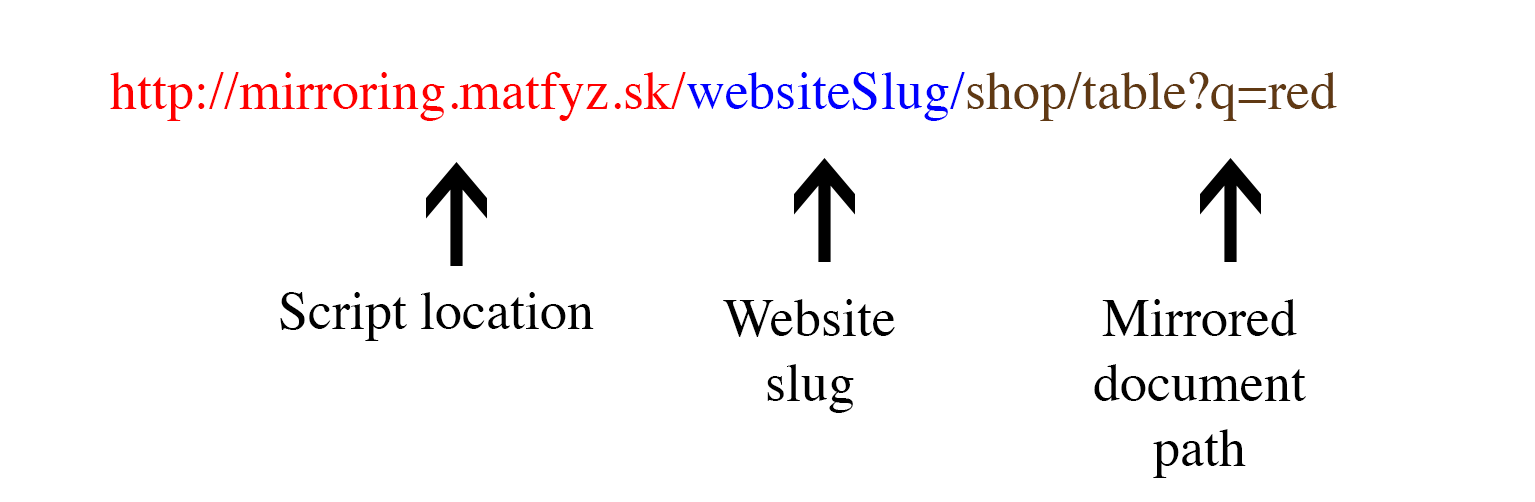
\includegraphics[width=\textwidth]{images/urls.png}
    \caption{Explanation of URL paths in serving of documents}
    \label{fig:urls}
\end{figure}

On Figure \ref{fig:urls} is shown how our serving script decides, which document to serve. First part of the URL is script location, then there is website slug. This slug is generally random generated UID to distinct between mirrored web pages. Then, the thirth part is a query for mirrored single document of a web page.

Now, the question is, how we can implement this URL management. As we described earlier, we can use Apache 2 Mod\_rewrite. This mod is generally used for rewriting URLs on server side and with a configuration script, we may force Apache 2 to always execute \texttt{index.php} script in our script directory. Used configuration, in form of \texttt{.htaccess} file is shown on Listing \ref{lst:htaccess}

\begin{lstlisting}[caption={Example of .htaccess for Apache 2 mod\_rewrite},label={lst:htaccess}]
RewriteEngine On
RewriteBase /
RewriteRule ^index\.php$ - [L]
RewriteCond %{REQUEST_FILENAME} !-f
RewriteCond %{REQUEST_FILENAME} !-d
RewriteRule . /index.php [L]
\end{lstlisting}

The last part of document serving is hidden inside \texttt{index.php} script saved in \texttt{webclone/server/index.php}. This script is executed for every request and its purpose is to extract website slug and query from document from an URL of request. Then, script loads requested data from database and tries to simulate the original response from the mirrored website even with its original status code.  This behaviour is shown on Listing \ref{lst:servingMirrored}.

\begin{lstlisting}[caption={Serving of mirrored documents},label={lst:servingMirrored}]

$uri = $_SERVER['REQUEST_URI'];

// delete first '/'
$uri = substr($uri, 1);

// split to slug and url
$pos = strpos($uri, '/');
$slug = substr($uri, 0, $pos);
$url = substr($uri, $pos+1);

$db = new Database();
$result = $db->getDocument($slug, $url);

// handle 200 OK
if ($result['http_code'] == 200) {
    $file =  WEBCLONE_ROOTDIR . $result['site_slug'] . '/' . $result['document_slug'];
    header("Content-Type: ".$result['content_type']);
    readfile($file);
    die();
} 
// handle REDIRECT
elseif ($result['http_code'] == 301 or $result['http_code'] == 302) {
    header("Location: ".$result['redirect_location']);
    die();
}
// handle ERROR
else {
    header("HTTP/1.0 404 Not Found");
    die();
}
\end{lstlisting}
